%% CA-SUS-HBF for Near-Field STAR-RIS Systems
%% Layout aligned with GA_HBF_STAR_RIS_presentation.tex
%%   pdflatex CA_SUS_STAR_RIS_presentation.tex
\documentclass[aspectratio=169,11pt]{beamer}

\usetheme{default}
\usecolortheme{default}
\setbeamertemplate{navigation symbols}{}

\definecolor{navyblue}{RGB}{0,51,102}
\definecolor{darkblue}{RGB}{0,51,102}
\definecolor{softblue}{RGB}{232,240,248}
\definecolor{softgreen}{RGB}{226,242,226}
\definecolor{notegreen}{RGB}{34,102,68}
\definecolor{titlebar}{RGB}{0,40,85}

\setbeamercolor{structure}{fg=navyblue}
\setbeamercolor{frametitle}{bg=navyblue,fg=white}
\setbeamercolor{title}{fg=black}
\setbeamercolor{block title}{bg=titlebar,fg=white}
\setbeamercolor{block body}{bg=softblue,fg=black}
\setbeamercolor{item}{fg=navyblue}
\setbeamerfont{frametitle}{size=\large}
\setbeamertemplate{itemize item}[circle]
\setbeamertemplate{bibliography item}[text]
\setbeamertemplate{caption}{\insertcaption}
\setbeamertemplate{footline}{}

\usepackage[T1]{fontenc}
\usepackage[utf8]{inputenc}
\usepackage{amsmath,amssymb,bm}
\usepackage{graphicx}
\usepackage{tikz}
\usetikzlibrary{arrows.meta,positioning,fit,calc}

\graphicspath{{presentation_figs/}}

\newcommand{\confbanner}{ATC 2026, 15--17 October 2026, Quy Nhon, Vietnam}
\newcommand{\confshort}{ATC 2026}
\newcommand{\conffull}{2026 International Conference on Advanced Technologies for Communications}

% Context card: bold lead-in + body, same size, one box (no title bar)
\newcommand{\ctxbox}[2]{%
  \noindent
  \begin{tikzpicture}
    \node[draw=navyblue, rounded corners, fill=softblue,
          inner sep=8pt, text width=0.92\textwidth, align=left] {
      {\normalsize\textbf{#1}}~{\normalsize #2}};
  \end{tikzpicture}\\[0.55em]}

\begin{document}

%======================================================================
% TITLE
%======================================================================
\begin{frame}[plain]
\gdef\slidefootnote{}
\begin{tikzpicture}[remember picture, overlay]
\fill[darkblue] (current page.north west) rectangle ([yshift=-3.2cm]current page.north east);
\node[white, font=\small\bfseries] at ([yshift=-0.45cm]current page.north)
    {\confbanner};
\node[white, font=\Large\bfseries] at ([yshift=-1.5cm]current page.north) {\confshort};
\node[white, font=\normalsize] at ([yshift=-2.5cm]current page.north)
    {\conffull};
\node[black, font=\large\bfseries, text width=0.94\textwidth, align=center]
    at ([yshift=-4.8cm]current page.north)
    {Conflict-Aware User Scheduling and Hybrid Beamforming\\
     for Near-Field STAR-RIS Systems};
\node[black, font=\small, text width=0.94\textwidth, align=center]
    at ([yshift=-6.5cm]current page.north)
    {Authors: Thuan Van Le, Hai Minh Truong, Ngo Hoang Tu,\\
     Vo Nguyen Quoc Bao, Nguyen Tien Hoa};
\node[black, font=\small\bfseries] at ([yshift=-7.5cm]current page.north)
    {Presented By: Hai Minh Truong};
\end{tikzpicture}
\end{frame}

%======================================================================
% CONTEXT
%======================================================================
\begin{frame}{1. Context \& Motivation}
  \ctxbox{STAR-RIS:}{A simultaneously transmitting and reflecting surface that covers both sides of space.
    Users only receive; T-side or R-side is decided by location.
    In this work the STAR coefficients are already set for the slot.}
  \ctxbox{Hybrid beamforming:}{The base station uses a limited number of RF chains, so only a few analog beams
    and a few users can be served in each slot.
    Each scheduled user is assigned one analog beam from a codebook, then a digital precoder.}
  \ctxbox{Constraint:}{The candidate pool is larger than the stream budget.
    In the near field, users whose effective channels point the same way at the BS
    fight for the same analog beam.
    Top-gain collides; plain semi-orthogonal selection drops useful users.}
\end{frame}

%======================================================================
% OVERALL ARCHITECTURE
%======================================================================
\begin{frame}{2. Overall Architecture}
  \begin{columns}[T,onlytextwidth]
    \begin{column}{0.56\textwidth}
      \centering
      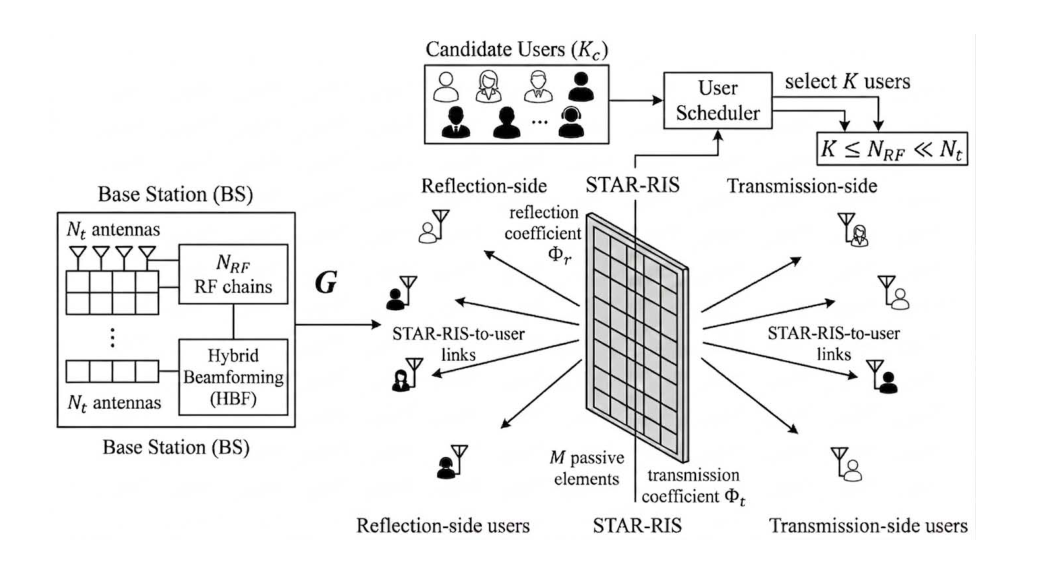
\includegraphics[width=\linewidth,height=0.62\textheight,keepaspectratio]{ref_star_ris.pdf}\\[0.2em]
      {\scriptsize STAR-RIS architecture}
    \end{column}
    \begin{column}{0.42\textwidth}
      \vspace{0.05em}
      {\footnotesize
      \begin{itemize}\setlength{\itemsep}{0.48em}
        \item \textbf{Limited hybrid stream budget}\\
        Few RF chains, so only $K$ users
        are served in one slot, and each
        of them gets one analog beam.
        \item \textbf{Conflict-aware user selection}\\
        Rank users by strength, beam conflict,
        and orthogonality, then grow a set
        whose analog directions stay apart.
        \item \textbf{STAR coefficients are an input}\\
        $\Phi_T$ and $\Phi_R$ are preconfigured;
        the panel only applies those coefs.
        The BS outputs $S$ and $F$, not a new surface.
      \end{itemize}}
    \end{column}
  \end{columns}
\end{frame}

%======================================================================
% SYSTEM MODEL
%======================================================================
\begin{frame}{3. System Model}
  \vspace{0.2cm}
  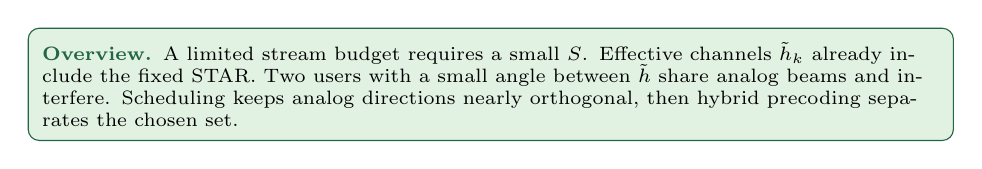
\begin{tikzpicture}
    \node[draw=notegreen, rounded corners, fill=softgreen,
          align=left, inner sep=5pt, text width=0.94\textwidth, font=\scriptsize] {
      \textbf{\color{notegreen}Overview.}
      A limited stream budget requires a small $S$.
      Effective channels $\tilde{h}_k$ already include the fixed STAR.
      Two users with a small angle between $\tilde{h}$ share analog beams and interfere.
      Scheduling keeps analog directions nearly orthogonal, then hybrid precoding
      separates the chosen set.};
  \end{tikzpicture}

  \vspace{-0.35cm}
  \begin{center}
  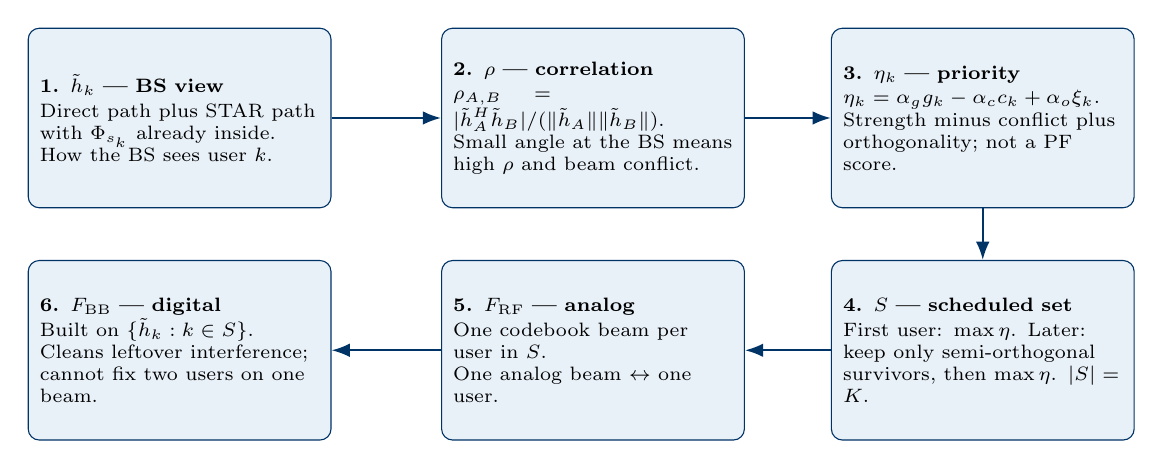
\begin{tikzpicture}[
      arr/.style={-{Latex}, thick, navyblue},
      card/.style={draw=navyblue, rounded corners, fill=softblue,
                   align=left, inner sep=4.2pt, font=\scriptsize,
                   text width=3.55cm, minimum height=2.28cm}
    ]
    \node[card] (c1) at (0,1.60) {%
      \textbf{1. $\tilde{h}_k$ --- BS view}\\[0.12em]
      Direct path plus STAR path
      with $\Phi_{s_k}$ already inside.\\
      How the BS sees user $k$.};
    \node[card] (c2) at (5.25,1.60) {%
      \textbf{2. $\rho$ --- correlation}\\[0.12em]
      $\rho_{A,B}=|\tilde{h}_A^H\tilde{h}_B|/(\|\tilde{h}_A\|\|\tilde{h}_B\|)$.\\
      Small angle at the BS means
      high $\rho$ and beam conflict.};
    \node[card] (c3) at (10.20,1.60) {%
      \textbf{3. $\eta_k$ --- priority}\\[0.12em]
      $\eta_k=\alpha_g g_k-\alpha_c c_k+\alpha_o\xi_k$.\\
      Strength minus conflict plus
      orthogonality; not a PF score.};
    \node[card] (c6) at (0,-1.35) {%
      \textbf{6. $F_{\mathrm{BB}}$ --- digital}\\[0.12em]
      Built on $\{\tilde{h}_k:k\in S\}$.\\
      Cleans leftover interference;
      cannot fix two users on one beam.};
    \node[card] (c5) at (5.25,-1.35) {%
      \textbf{5. $F_{\mathrm{RF}}$ --- analog}\\[0.12em]
      One codebook beam per user in $S$.\\
      One analog beam $\leftrightarrow$ one user.};
    \node[card] (c4) at (10.20,-1.35) {%
      \textbf{4. $S$ --- scheduled set}\\[0.12em]
      First user: $\max\eta$. Later: keep
      only semi-orthogonal survivors,
      then $\max\eta$. $|S|=K$.};

    \draw[arr] (c1)--(c2);
    \draw[arr] (c2)--(c3);
    \draw[arr] (c3)--(c4);
    \draw[arr] (c4)--(c5);
    \draw[arr] (c5)--(c6);
  \end{tikzpicture}
  \end{center}
\end{frame}

%======================================================================
% PROPOSED
%======================================================================
\begin{frame}{4. Proposed CA-SUS-HBF Scheme}
  \vspace{0.2cm}
  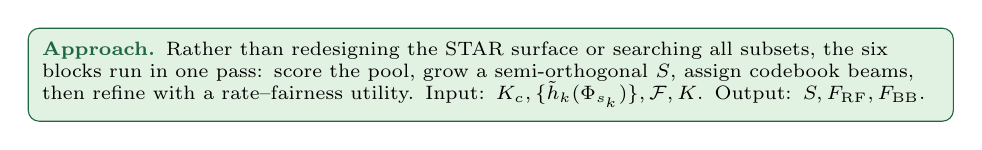
\begin{tikzpicture}
    \node[draw=notegreen, rounded corners, fill=softgreen,
          align=left, inner sep=5pt, text width=0.94\textwidth, font=\scriptsize] {
      \textbf{\color{notegreen}Approach.}
      Rather than redesigning the STAR surface or searching all subsets,
      the six blocks run in one pass: score the pool, grow a semi-orthogonal $S$,
      assign codebook beams, then refine with a rate--fairness utility.
      Input: $K_c,\{\tilde{h}_k(\Phi_{s_k})\},\mathcal{F},K$.
      Output: $S,F_{\mathrm{RF}},F_{\mathrm{BB}}$.};
  \end{tikzpicture}

  \vspace{-0.35cm}
  \begin{center}
  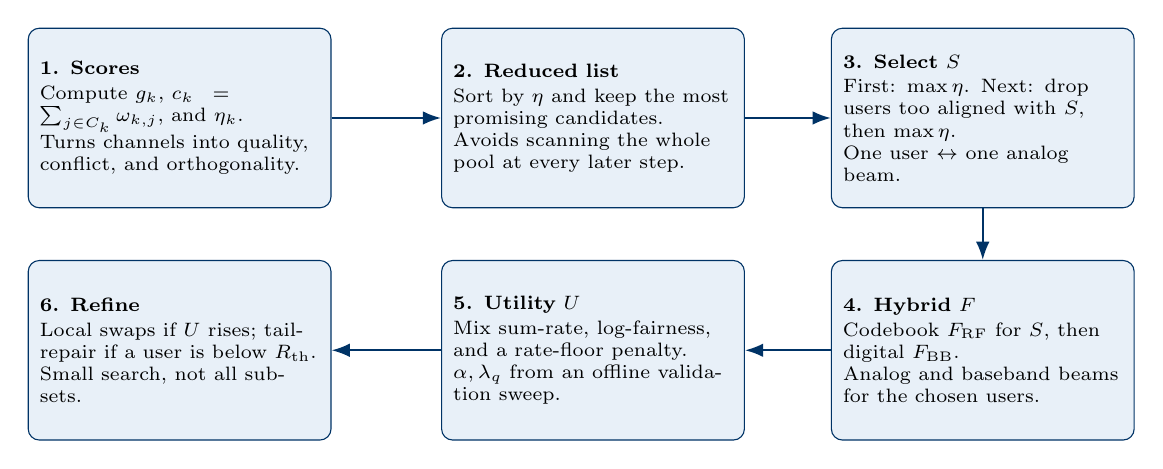
\begin{tikzpicture}[
      arr/.style={-{Latex}, thick, navyblue},
      card/.style={draw=navyblue, rounded corners, fill=softblue,
                   align=left, inner sep=4.2pt, font=\scriptsize,
                   text width=3.55cm, minimum height=2.28cm}
    ]
    \node[card] (c1) at (0,1.60) {%
      \textbf{1. Scores}\\[0.12em]
      Compute $g_k$, $c_k=\sum_{j\in C_k}\omega_{k,j}$,
      and $\eta_k$.\\
      Turns channels into quality,
      conflict, and orthogonality.};
    \node[card] (c2) at (5.25,1.60) {%
      \textbf{2. Reduced list}\\[0.12em]
      Sort by $\eta$ and keep the
      most promising candidates.\\
      Avoids scanning the whole pool
      at every later step.};
    \node[card] (c3) at (10.20,1.60) {%
      \textbf{3. Select $S$}\\[0.12em]
      First: $\max\eta$. Next: drop users
      too aligned with $S$, then $\max\eta$.\\
      One user $\leftrightarrow$ one analog beam.};
    \node[card] (c6) at (0,-1.35) {%
      \textbf{6. Refine}\\[0.12em]
      Local swaps if $U$ rises;
      tail-repair if a user is below $R_{\mathrm{th}}$.\\
      Small search, not all subsets.};
    \node[card] (c5) at (5.25,-1.35) {%
      \textbf{5. Utility $U$}\\[0.12em]
      Mix sum-rate, log-fairness,
      and a rate-floor penalty.\\
      $\alpha,\lambda_q$ from an offline
      validation sweep.};
    \node[card] (c4) at (10.20,-1.35) {%
      \textbf{4. Hybrid $F$}\\[0.12em]
      Codebook $F_{\mathrm{RF}}$ for $S$,
      then digital $F_{\mathrm{BB}}$.\\
      Analog and baseband beams
      for the chosen users.};

    \draw[arr] (c1)--(c2);
    \draw[arr] (c2)--(c3);
    \draw[arr] (c3)--(c4);
    \draw[arr] (c4)--(c5);
    \draw[arr] (c5)--(c6);
  \end{tikzpicture}
  \end{center}
\end{frame}

%======================================================================
% SIMULATION --- paper captions only
%======================================================================
\begin{frame}{5. Simulation Results (Rate)}
  \begin{columns}[T,onlytextwidth]
    \begin{column}{0.48\textwidth}
      \centering
      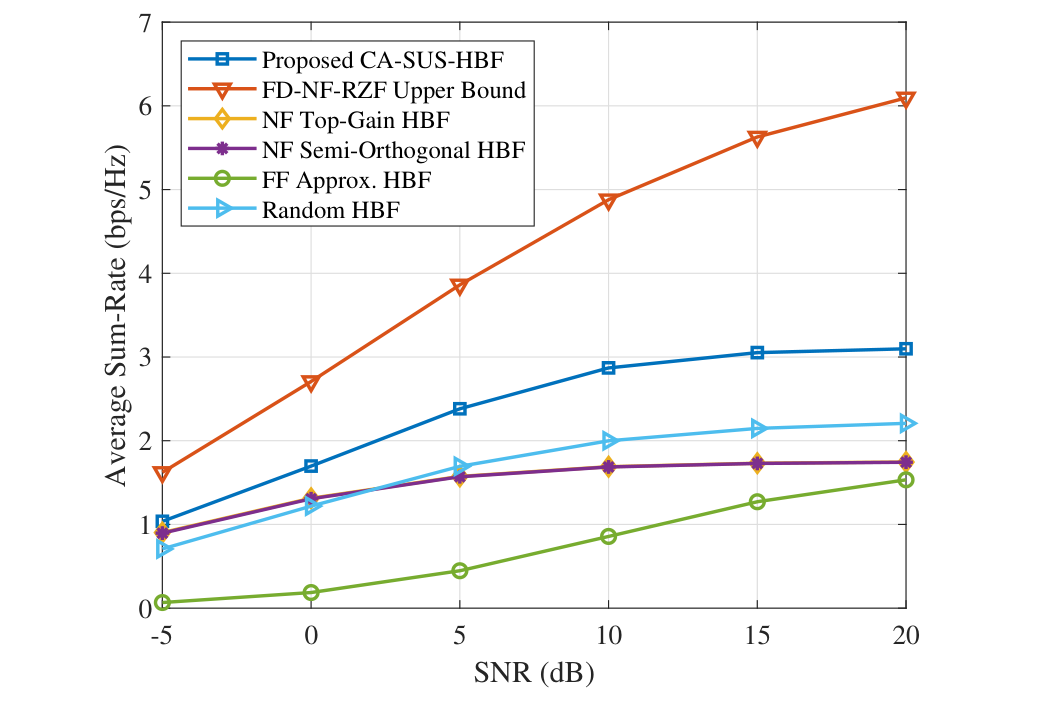
\includegraphics[width=0.99\linewidth]{fig1.pdf}\\[0.15em]
      {\scriptsize Figure 1. Average sum-rate versus SNR for different HBF schemes
      in the considered near-field STAR-RIS systems.}
    \end{column}
    \begin{column}{0.48\textwidth}
      \centering
      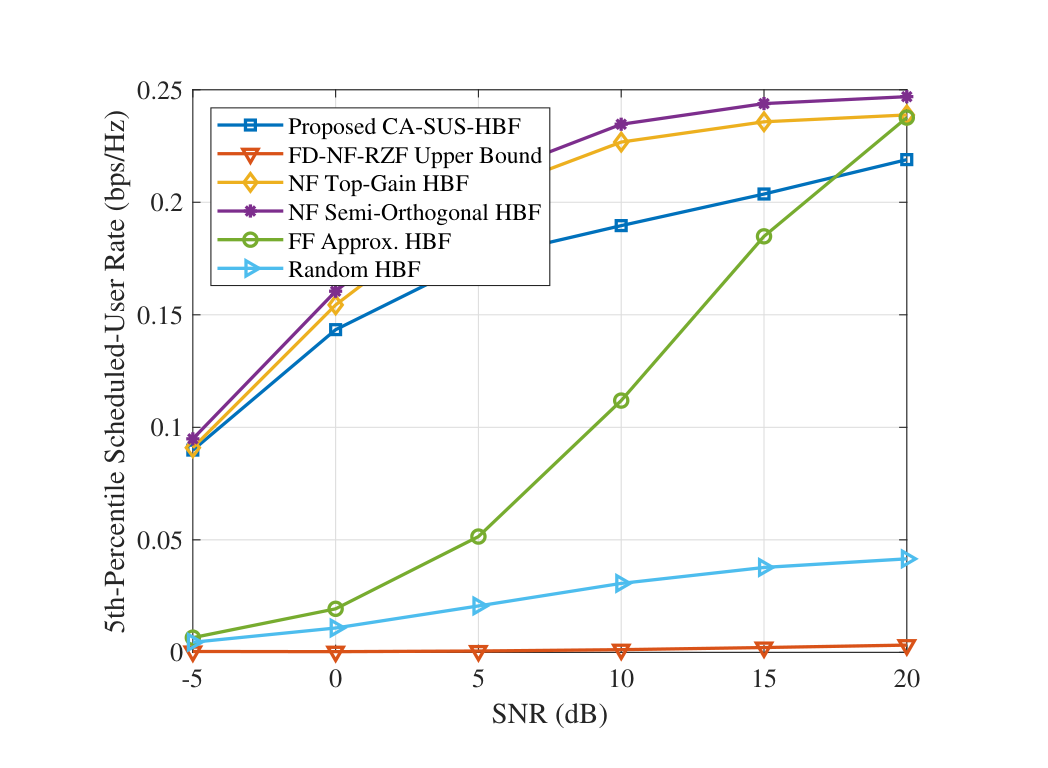
\includegraphics[width=0.99\linewidth]{fig2.pdf}\\[0.15em]
      {\scriptsize Figure 2. 5th-percentile scheduled-user rate versus SNR for different
      HBF schemes in the considered near-field STAR-RIS system.}
    \end{column}
  \end{columns}
\end{frame}

\begin{frame}{6. Simulation Results (Users and Fairness)}
  \begin{columns}[T,onlytextwidth]
    \begin{column}{0.48\textwidth}
      \centering
      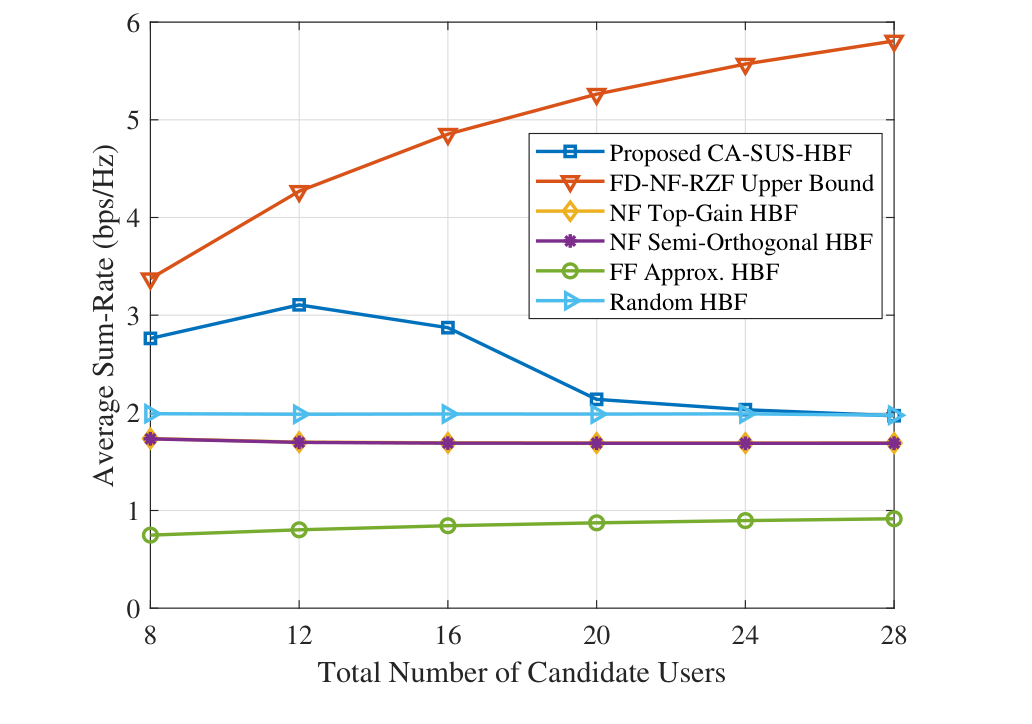
\includegraphics[width=0.99\linewidth]{fig3.pdf}\\[0.15em]
      {\scriptsize Figure 3. Average sum-rate versus the total number of candidate users.}
    \end{column}
    \begin{column}{0.48\textwidth}
      \centering
      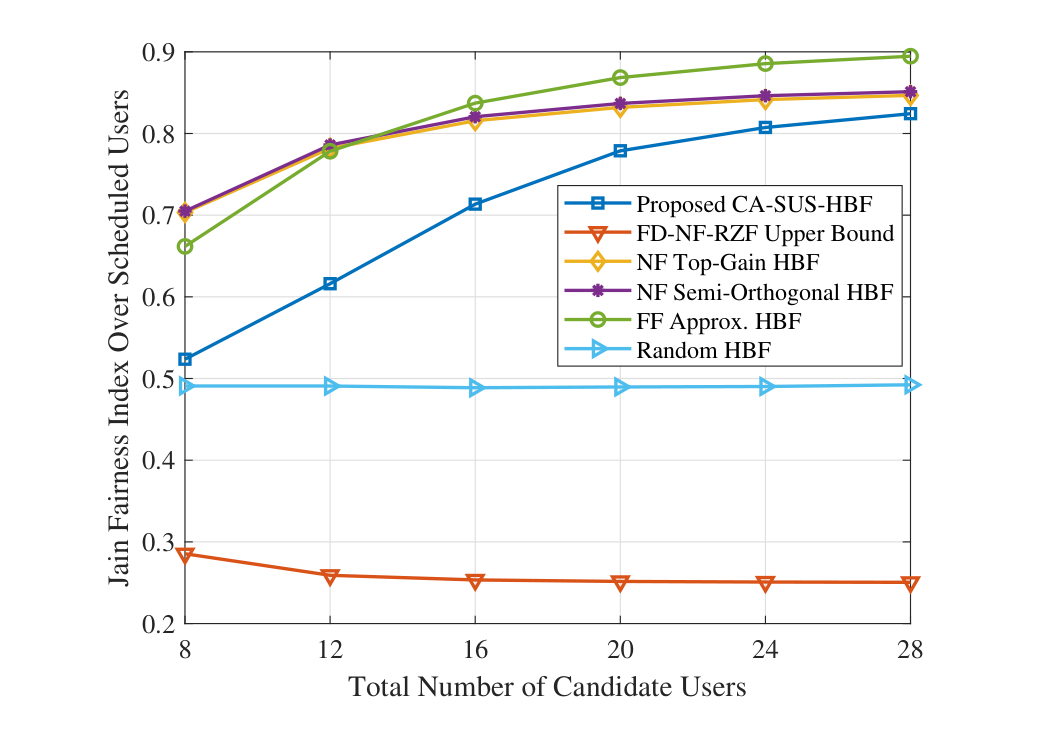
\includegraphics[width=0.99\linewidth]{fig4.pdf}\\[0.15em]
      {\scriptsize Figure 4. Jain's fairness index versus the total number of candidate users.}
    \end{column}
  \end{columns}
\end{frame}

%======================================================================
% REFERENCES
%======================================================================
\begin{frame}{7. References}
\fontsize{6.1pt}{7.15pt}\selectfont
\begin{thebibliography}{15}
\bibitem{guirado}
R.~Guirado, R.~Verdecia-Pe\~{n}a, G.~Perez-Palomino, E.~Carrasco, and J.~I.~Alonso,
``Prototype and performance assessment of mmWave active RIS-enhanced 6G communications,''
\textit{IEEE Trans.\ Green Commun.\ Netw.}, vol.~10, pp.~412--425, 2026.
\bibitem{wu_zhang_irs}
Q.~Wu and R.~Zhang,
``Intelligent reflecting surface enhanced wireless network via joint active and passive beamforming,''
\textit{IEEE Trans.\ Wireless Commun.}, vol.~18, no.~11, pp.~5394--5409, 2019.
\bibitem{mu_star}
X.~Mu, Y.~Liu, L.~Guo, J.~Lin, and R.~Schober,
``Simultaneously transmitting and reflecting (STAR) RIS aided wireless communications,''
\textit{IEEE Trans.\ Wireless Commun.}, vol.~21, no.~5, pp.~3083--3098, 2022.
\bibitem{khalid}
W.~Khalid, Z.~Kaleem, R.~Ullah, T.~Van Chien, S.~Noh, and H.~Yu,
``Simultaneous transmitting and reflecting-reconfigurable intelligent surface in 6G: Design guidelines and future perspectives,''
\textit{IEEE Netw.}, vol.~37, no.~5, pp.~173--181, 2023.
\bibitem{ayach}
O.~E.~Ayach, S.~Rajagopal, S.~Abu-Surra, Z.~Pi, and R.~W.~Heath,
``Spatially sparse precoding in millimeter wave MIMO systems,''
\textit{IEEE Trans.\ Wireless Commun.}, vol.~13, no.~3, pp.~1499--1513, 2014.
\bibitem{molisch}
A.~F.~Molisch, V.~V.~Ratnam, S.~Han, Z.~Li, S.~L.~H.~Nguyen, L.~Li, and K.~Haneda,
``Hybrid beamforming for massive MIMO: A survey,''
\textit{IEEE Commun.\ Mag.}, vol.~55, no.~9, pp.~134--141, 2017.
\bibitem{dao}
H.~T.~Dao and S.~Kim,
``Effective channel gain-based access point selection in cell-free massive MIMO systems,''
\textit{IEEE Access}, vol.~8, pp.~108127--108132, 2020.
\bibitem{mao_sus}
J.~Mao, J.~Gao, Y.~Liu, and G.~Xie,
``Simplified semi-orthogonal user selection for MU-MIMO systems with ZFBF,''
\textit{IEEE Wireless Commun.\ Lett.}, vol.~1, no.~1, pp.~42--45, 2012.
\bibitem{yoo}
T.~Yoo and A.~Goldsmith,
``On the optimality of multiantenna broadcast scheduling using zero-forcing beamforming,''
\textit{IEEE J.\ Sel.\ Areas Commun.}, vol.~24, no.~3, pp.~528--541, 2006.
\bibitem{wu_zhang_env}
Q.~Wu and R.~Zhang,
``Towards smart and reconfigurable environment: Intelligent reflecting surface aided wireless network,''
\textit{IEEE Commun.\ Mag.}, vol.~58, no.~1, pp.~106--112, 2020.
\bibitem{peel}
C.~Peel, B.~Hochwald, and A.~Swindlehurst,
``A vector-perturbation technique for near-capacity multiantenna multiuser communication--part I: channel inversion and regularization,''
\textit{IEEE Trans.\ Commun.}, vol.~53, no.~1, pp.~195--202, 2005.
\end{thebibliography}
\end{frame}

\begin{frame}[plain]
\begin{tikzpicture}[remember picture, overlay]
    \fill[navyblue] (current page.south west) rectangle (current page.north east);
\end{tikzpicture}
\vspace{1.5cm}
\begin{center}
    \textcolor{white}{\Huge\textbf{Thank You}}\\[0.8cm]
    \textcolor{white}{\small \confshort~$\bullet$~Quy Nhon}
\end{center}
\end{frame}

\end{document}
